% --- SLIDE 8: CONCEPT DEVELOPMENT (DINAMICA) ---
\begin{frame}{Concept Development: Smart Dynamic Response of STF}

    \vspace{-0.3cm}
    % --- NUOVA SEZIONE CON IMMAGINE CENTRATA ---
    % Sostituisci 'percorso_della_tua_immagine' con il file reale
    % Puoi regolare width o scale per ottimizzare la dimensione
    \begin{center}
        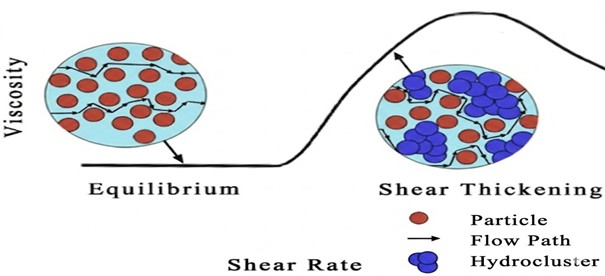
\includegraphics[width=0.45\textwidth,keepaspectratio]{image/graficoSTF.jpg}
    \end{center}
    % ---------------------------------------------

    \vspace{-0.45cm} % Spazio verticale ridotto leggermente per bilanciare con l'immagine

    \begin{columns}[T]
        % Box Sinistra: Camminata
        \begin{column}{0.48\textwidth}
            \begin{alertblock}{Low Shear Rate (Walk, $Fr < 0.5$)}
                \begin{itemize}
                    \item \textbf{STF State:} Low viscosity (Fluid).
                    \item \textbf{Mechanics:} The TPMS matrix deforms elastically under the load.
                    \item \textbf{Cushioning:} The heel "sinks" to absorb terrain irregularities.
                    \item \textbf{Result:} Natural \textit{roll-over}, optimal damping without triggering the stiff blade.
                \end{itemize}
            \end{alertblock}
        \end{column}

        % Box Destra: Corsa
        \begin{column}{0.48\textwidth}
            \begin{exampleblock}{High Shear Rate (Run, $Fr > 0.5$)}
                \begin{itemize}
                    \item \textbf{STF State:} Instant solidification.
                    \item \textbf{Mechanics:} The damper locks its volumetric deformation.
                    \item \textbf{Bridging:} The heel becomes a rigid bridge, dissipating zero energy.
                    \item \textbf{Result:} Ground Reaction Forces (GRF) are fully transferred to the blade for propulsion.
                \end{itemize}
            \end{exampleblock}
        \end{column}
    \end{columns}
\end{frame}